\documentclass[10pt]{beamer}
\usepackage{graphicx}
\usepackage{adjustbox}
\usepackage{hyperref}
\usepackage{amsmath}
\usepackage{hyperref}
\usepackage{graphicx}
\usepackage{float}
\usepackage{caption}
\usepackage{listings}
\usepackage{xcolor}


% Define colors
\colorlet{punct}{red!60!black}
\definecolor{background}{RGB}{240, 248, 255} % Pale Blue
\definecolor{delim}{RGB}{20,105,176}
\colorlet{numb}{magenta!60!black}

% Define JSON language
\lstdefinelanguage{json}{
    basicstyle=\normalfont\ttfamily,
    numbers=left,
    numberstyle=\scriptsize,
    stepnumber=1,
    numbersep=8pt,
    showstringspaces=false,
    breaklines=true,
    frame=lines,
    backgroundcolor=\color{background},
    literate=
     *{0}{{{\color{numb}0}}}{1}
      {1}{{{\color{numb}1}}}{1}
      {2}{{{\color{numb}2}}}{1}
      {3}{{{\color{numb}3}}}{1}
      {4}{{{\color{numb}4}}}{1}
      {5}{{{\color{numb}5}}}{1}
      {6}{{{\color{numb}6}}}{1}
      {7}{{{\color{numb}7}}}{1}
      {8}{{{\color{numb}8}}}{1}
      {9}{{{\color{numb}9}}}{1}
      {:}{{{\color{punct}{:}}}}{1}
      {,}{{{\color{punct}{,}}}}{1}
      {\{}{{{\color{delim}{\{}}}}{1}
      {\}}{{{\color{delim}{\}}}}}{1}
      {[}{{{\color{delim}{[}}}}{1}
      {]}{{{\color{delim}{]}}}}{1},
}


\usetheme{Copenhagen}
\usecolortheme{default}  % You can choose from various color themes provided by metropolis
% \setbeamertemplate{footline}[frame number]
\setbeamertemplate{navigation symbols}{}

\title[exMA WP1 Vegetation]{
  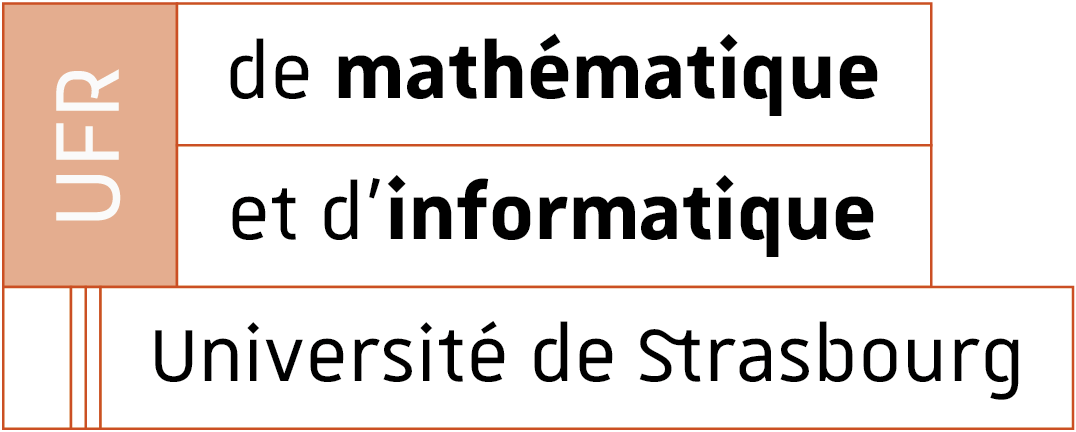
\includegraphics[width=0.8\textwidth]{images/logo_ufr.png}
  Project WP1 - Vegetation}
\author[PA-Giulio]{Giulio CARPI LAPI, Pierre-Antoine SENGER}

\begin{document}

\frame{\titlepage}

\begin{frame}{Context : Impact of vegetation on urban heat}
  \begin{figure}[H]
    \centering
    \begin{minipage}{0.49\textwidth}
        \centering
        \includegraphics[width=\textwidth]{images/TreeShade.png}
        \captionsetup{font={scriptsize}}
        \caption{Tree providing shade to a building \cite{img:TreeShade}.}
    \end{minipage}\hfill
    \begin{minipage}{0.49\textwidth}
        \centering
        \includegraphics[width=\textwidth]{images/heat_street.png}
        \captionsetup{font={scriptsize}}
        \caption{Thermal image of a street depicting heat distribution \cite{img:street_thermography}.}
    \end{minipage}
  \end{figure}
\end{frame}

\begin{frame}{Objectives}
  \begin{figure}[H]
    \centering
    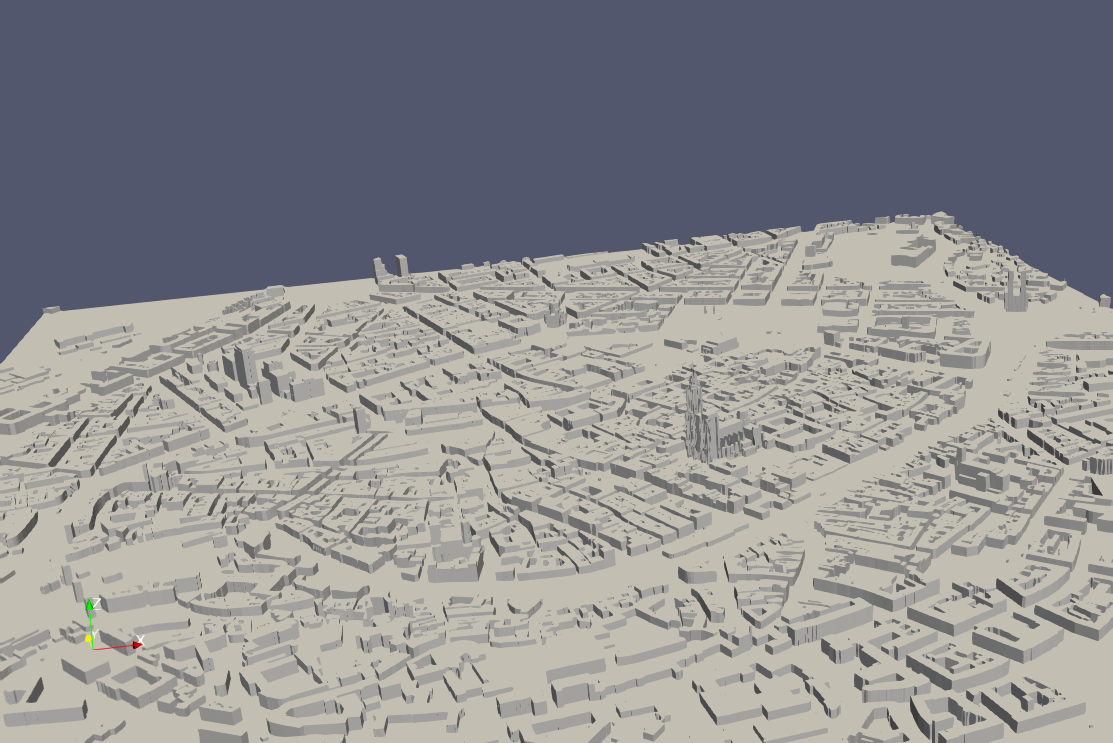
\includegraphics[width=1\textwidth]{images/stras_mesh.png}
    \captionsetup{font={scriptsize}}
    \caption{Strasbourg 3D model.}
  \end{figure}
\end{frame}

\begin{frame}{Objectives}
  Main objectives : run \textbf{sun masks} and \textbf{fluid mechanics} simulations using Feel++\cite{feel++} \\
  \vspace{0.5cm}

  \begin{itemize}
    \item<2-> \textbf{Sun masks} : compute the shadow cast by trees on the ground and buildings
    \item<3-> \textbf{Fluid mechanics} : simulate the air flow around trees
  \end{itemize}
\end{frame}

\begin{frame}{Starting point}
  We have :
  \begin{itemize}
    \item<2-> some scientific articles \cite{Verdie14} \cite{Verdie15} \cite{Stava14} ...
    \item <3-> CGAL\cite{cgal} C++ library to mesh trees \includegraphics[width=0.2\textwidth]{images/cgal_logo.png}
    \item <4-> Feel++\cite{feel++} C++ library to run simulations 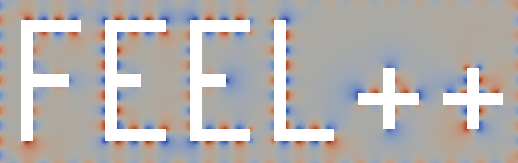
\includegraphics[width=0.2\textwidth]{images/feelpp.png}
    \item <5-> The 3D model of Strasbourg
  \end{itemize}
\end{frame}

\begin{frame}{Methodology: data acquisition}
  Use \textbf{OpenStreetMap} API to get the data about the trees in Strasbourg.

  \begin{figure}[H]
    \centering
    \begin{minipage}{0.49\textwidth}
        \centering
        
\includegraphics[width=\textwidth]{images/osm_logo.png}
        \captionsetup{font={scriptsize}}
        \caption{Overpass logo.}
    \end{minipage}\hfill
    \begin{minipage}{0.49\textwidth}
        \centering
        \includegraphics[width=\textwidth]{images/OvAPI_logo.png}
        \captionsetup{font={scriptsize}}
        \caption{Overpass API logo.}
    \end{minipage}
  \end{figure}
\end{frame}

\begin{frame}{Data acquisition: how API works}
  \begin{figure}[H]
    \centering
    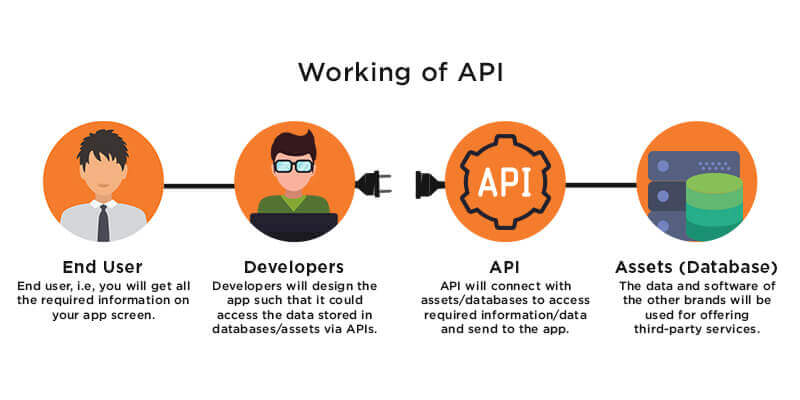
\includegraphics[width=1\textwidth]{images/how-api-works.jpg}
    \captionsetup{font={scriptsize}}
    \caption{Example of query to get trees in Strasbourg.}
  \end{figure}
\end{frame}

\begin{frame}{Data acquisition: Overpass turbo}
\href{https://overpass-turbo.eu/}{Overpass turbo}
 is a web-based data filtering tool for OpenStreetMap. 
It runs queries on the Overpass API.

  \begin{figure}[H]
    \centering
    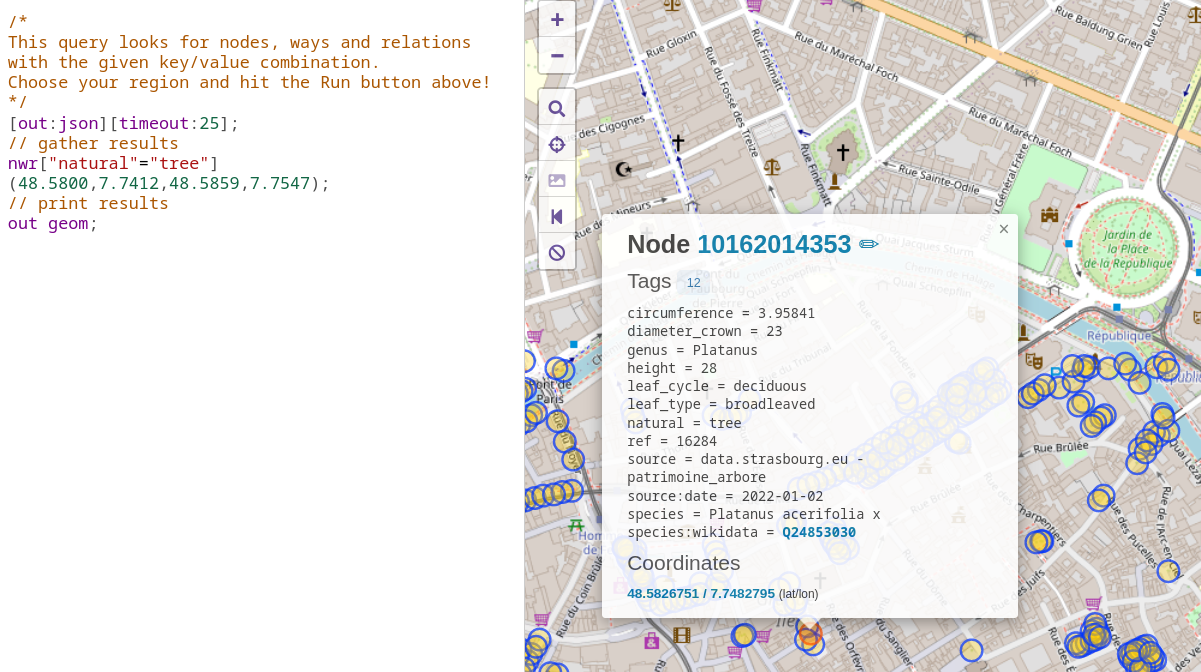
\includegraphics[width=1\textwidth]{images/overpass_turbo.png}
    \captionsetup{font={scriptsize}}
    \caption{Example of query to get trees in Strasbourg using Overpass turbo.}
  \end{figure}
\end{frame}

\begin{frame}[fragile]{Data acquisition: Curl}
  
\includegraphics[width=0.2\textwidth]{images/Curl-logo.svg.png}is a command-line tool to transfer data with URL syntax.
  We're using a configuration file \texttt{config.json} to specify the query parameters.
  Here is an example of a configuration file:
\begin{lstlisting}[language=json]
{
  "bbox": "48.5866,7.7522,48.5876,7.7557",
  "origin": "48.583055227464364, 7.748664426560083",
  "LOD": 0,
  "default_height_range": "3, 40",
  "default_genus": "Platanus",
  "input_building_mesh": "mesh_lod1.stl",
  "output_name": "republique"
}
\end{lstlisting}
\end{frame}

\begin{frame}[fragile]{Data acquisition: Curl - Query result} 
  The result of the query is a JSON file \texttt{query\_result.json} containing the data about the trees.
Here is the beginning of the file from the previous query:

\begin{lstlisting}[language=json]
{
  "version": 0.6,
  "generator": "Overpass API 0.7.62.1 084b4234",
  "osm3s": {
    "timestamp_osm_base": "2024-05-26T13:31:45Z",
    "copyright": "The data included in this document is from www.openstreetmap.org. The data is made available under ODbL."
  },
  "elements": [
\end{lstlisting}
\end{frame}

\begin{frame}[fragile]{Data acquisition: Curl - Query result}
 The elements are the trees:

\begin{lstlisting}[language=json]
{
  "type": "node",
  "id": 10161978687,
  "lat": 48.5871937,
  "lon": 7.7531245,
  "tags": {
    "circumference": "0.62832",
    "diameter_crown": "5",
    "genus": "Tilia",
    "height": "9",
    "natural": "tree",
    "ref": "27490",
    "source": "data.strasbourg.eu - patrimoine_arbore",
    "source:date": "2022-01-02",
    "species": "Tilia euchlora x"
  }
}, ...
\end{lstlisting}
\end{frame}

\begin{frame}[fragile]{Data acquisition: Curl - Query result}
  A tree with less information:

\begin{lstlisting}[language=json]
{
    "type": "node",
    "id": 4439566691,
    "lat": 48.5839128,
    "lon": 7.7487125,
    "tags": {
      "natural": "tree"
    }
}
\end{lstlisting}

\end{frame}



% \nocite{*}
\bibliographystyle{plain}
\bibliography{references}

\end{document}